\chapter{Evaluation}\label{chapter:evaluation}
In order to show that the CloudASR platform is ready for the production usage
  several benchmarks were made.
First, real time factor (RTF) of the batch speech recognition mode was measured and compared with Google Speech API.
Second, latency of the online speech recognition mode was measured.
Finally, number of parallel requests for batch speech recognition mode was measured.
These benchmarks will be described in the following section.


\section{RTF of Batch Speech Recognition}
In the first benchmark RTF of CloudASR batch mode was compared with RTF of Google Speech API
  using test set from the Czech Public Transportation Information Domain \cite{korvas2014vystadial}.
WER and RTF of both APIs were measured with following results:
Google Speech API had 60\% WER and RTF 0.3 whereas
  CloudASR had 22\% WER and RTF 0.22.
Request times of both APIs are displayed in Figure~\ref{fig:batch-benchmark}.

This benchmark shows that RTF of CloudASR batch mode is better than RTF of Google Speech API.
Moreover, the benchmark shows that the CloudASR platform can achieve better accuracy than Google Speech API on limitted domains
  if the used decoding graphs are customized for that domains.


\begin{figure}[h]
  \centering
  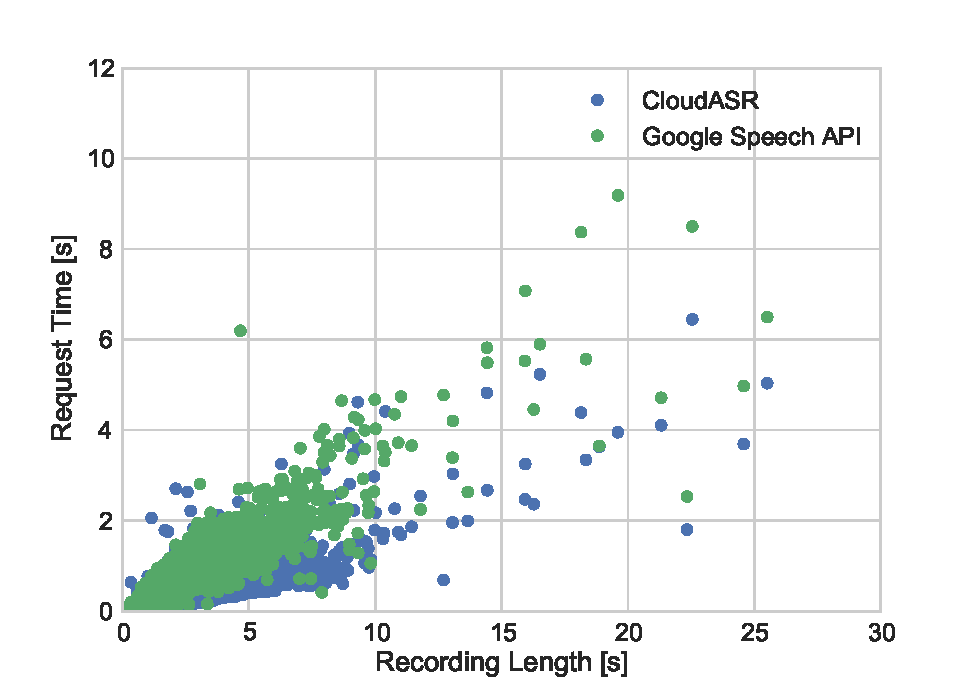
\includegraphics[width=0.75\textwidth]{./img/batch.pdf}

  \caption{
    Batch recognition benchmark.
  }
  \label{fig:batch-benchmark}
\end{figure}



\section{Latency of Online Speech Recognition}
In the second benchmark latency of CloudASR online mode was measured.
Since the low latency is crucial for successfull usage of speech recognition in dialogue systems
  and there are not so many webservice that provide online speech recognition mode
  support for online speech recognition mode can be seen as a key feature of the CloudASR platform.
The reason why the online speech recognition mode is better suited for dialogue systems is
  that it is not neccessary to wait for the whole recording to be recorded
  and instead it is possible to get the interim results while the speech is recorded.
Thus, dialogue systems can react quickly.
Figure~\ref{fig:online-benchmark} shows comparison of the deelay between utterance end and the availability of the recognition results for CloudASR online and batch mode.

\TODO{add conclusion}

\begin{figure}[h]
  \centering
  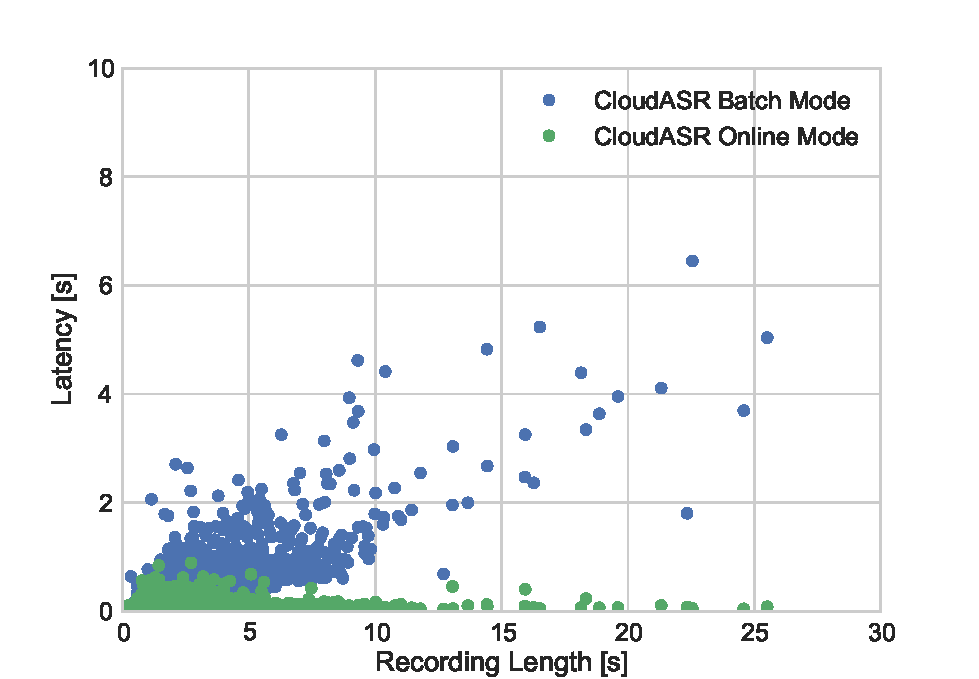
\includegraphics[width=0.75\textwidth]{./img/online.pdf}

  \caption{
    A latency comparison for CloudASR online and batch mode.
  }
  \label{fig:online-benchmark}
\end{figure}


\section{Parallel Requests Benchmark}
Since the main bottleneck of the CloudASR platform is a number of running workers
  workers with dummy asr engine (described in Figure~\ref{fig:dummyasr})
  that would enable to test how many parallel requests can CloudASR handle were used.
As a result, 1000 dummy workers could run on a Mesos cluster with 5 slaves (4CPU, 16GB RAM).
Also, HAProxy load-balancer, which spread workload accross 5 frontend containers, was deployed.

Then several benchmarks were run to show how RTF of the batch recognition mode changes with different number of parallel requests.
The platform was tested with a different number of parallel requests (50, 250, 500, 750 and 1000)
  and with files with different lengths (5s, 10s, 20s, 30s, 40s, 50s and 60s).
Results are summarized on Figure~\ref{fig:parallel-benchmark}.

Results show that CloudASR platform adds just a very little overhead compared to the raw dummy worker.
Moreover, results shows that the platform is able to handle much more parallel requests with appropriate number of workers.

\IDEA{Add benchmark code}
\IDEA{Network capacity, similarity to online recognition}
\IDEA{Add table with numbers}

\begin{figure}
  \centering
  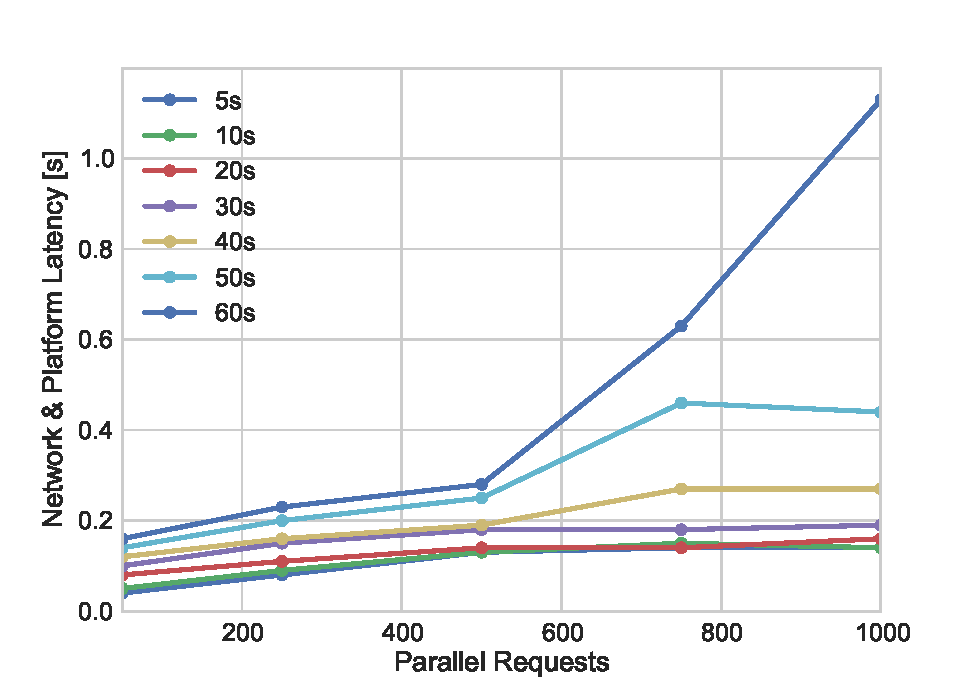
\includegraphics[width=0.75\textwidth]{./img/parallel.pdf}

  \caption{
    The graph shows platform \& network latency for recordings with various lengths
      given the number of parallel requests.
  }
  \label{fig:parallel-benchmark}
\end{figure}
